\section{Harmonische und Spektralanalyse bei Umrichtern}

Diese Section behandelt die \textbf{Harmonischen} und die \textbf{Spektralanalyse}
nichtsinusförmiger Spannungen und Ströme bei Leistungselektronik-Umrichtern.
Sie ist zentral für die Bewertung von \textbf{Verlusten}, \textbf{Filterbedarf},
\textbf{Netzrückwirkungen} und \textbf{Qualitätskennzahlen} wie THD.

\smallskip

\textbf{Zielbild:}
\begin{itemize}
    \item Entstehung von Harmonischen verstehen
    \item Fourier-Zerlegung von Umrichtersignalen anwenden
    \item Spektrum qualitativ interpretieren
    \item Verzerrungskennzahlen korrekt berechnen
\end{itemize}
\subsection*{Definition der verwendeten Grössen}

\begin{itemize}
    \item $U_{n,\mathrm{RMS}}$: Effektivwert der Harmonischen Ordnung $n$,
    \item $U_{1,\mathrm{RMS}}$: Effektivwert der Grundschwingung,
    \item $U_{\mathrm{RMS}}$: Gesamt-Effektivwert,
    \item $f_1$: Grundfrequenz,
    \item $f_c$: Schaltfrequenz,
    \item $\varphi_1$: Phasenwinkel der Grundschwingung,
    \item $\mathrm{THD}$: Total Harmonic Distortion,
    \item $\nu$: Verzerrungsfaktor.
\end{itemize}

\subsection{Ursprung der Harmonischen}

In Umrichtern entstehen Harmonische durch:
\begin{itemize}
    \item Schaltvorgänge
    \item Stückweise konstante Spannungen
    \item Phasenanschnittsteuerung
    \item Rechteck- und PWM-Spannungen
\end{itemize}

Grundprinzip:
\[
\cbl{\text{Jedes periodische, nichtsinusförmige Signal } \Rightarrow \text{ Summe aus Sinusschwingungen}.}
\]

\subsection{Allgemeine Harmonische und Spektralanalyse}

Fourier-Reihe:
\[
x(t) = a_0 + \sum_{k=1}^\infty 
\big( a_k \cos k\omega t + b_k \sin k\omega t \big)
\]

Grundfrequenz:
\[
f_1 = \frac{1}{T}
\]

Effektivwert aus Spektrum:
\[
X_{\mathrm{rms}}^2 = \sum_{k=1}^\infty X_{k,\mathrm{rms}}^2
\]

Dominante Harmonische bei PWM:
\[
f = m f_c \pm n f_1,
\qquad m,n \in \mathbb{N}
\]

\subsection{Fourier-Zerlegung}

Für ein $T$-periodisches Signal:
\[
\cbl{u(t) = \frac{a_0}{2} + \sum_{n=1}^{\infty}
\left[ a_n \cos(n \omega t) + b_n \sin(n \omega t) \right].}
\]

Mit:
\[
\omega = \frac{2\pi}{T}.
\]

Bedeutung:
\begin{itemize}
    \item $n=1$: Grundschwingung
    \item $n>1$: Harmonische Ordnung $n$
\end{itemize}


\subsection{Typische Spektren bei Umrichtern}

\subsubsection{Phasenanschnitt (Wechselstromsteller, B2C)}
\begin{center}
    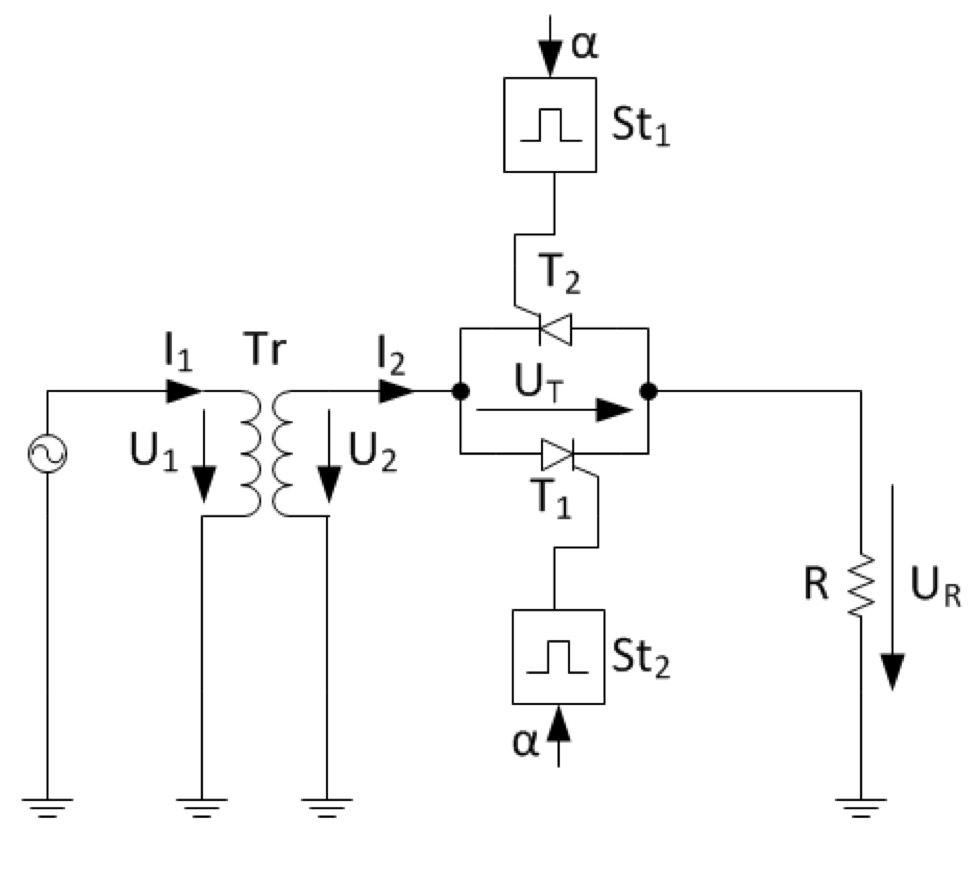
\includegraphics[width=0.85\linewidth]{images/Wechselstromsteller.png}
\end{center}

\begin{center}
    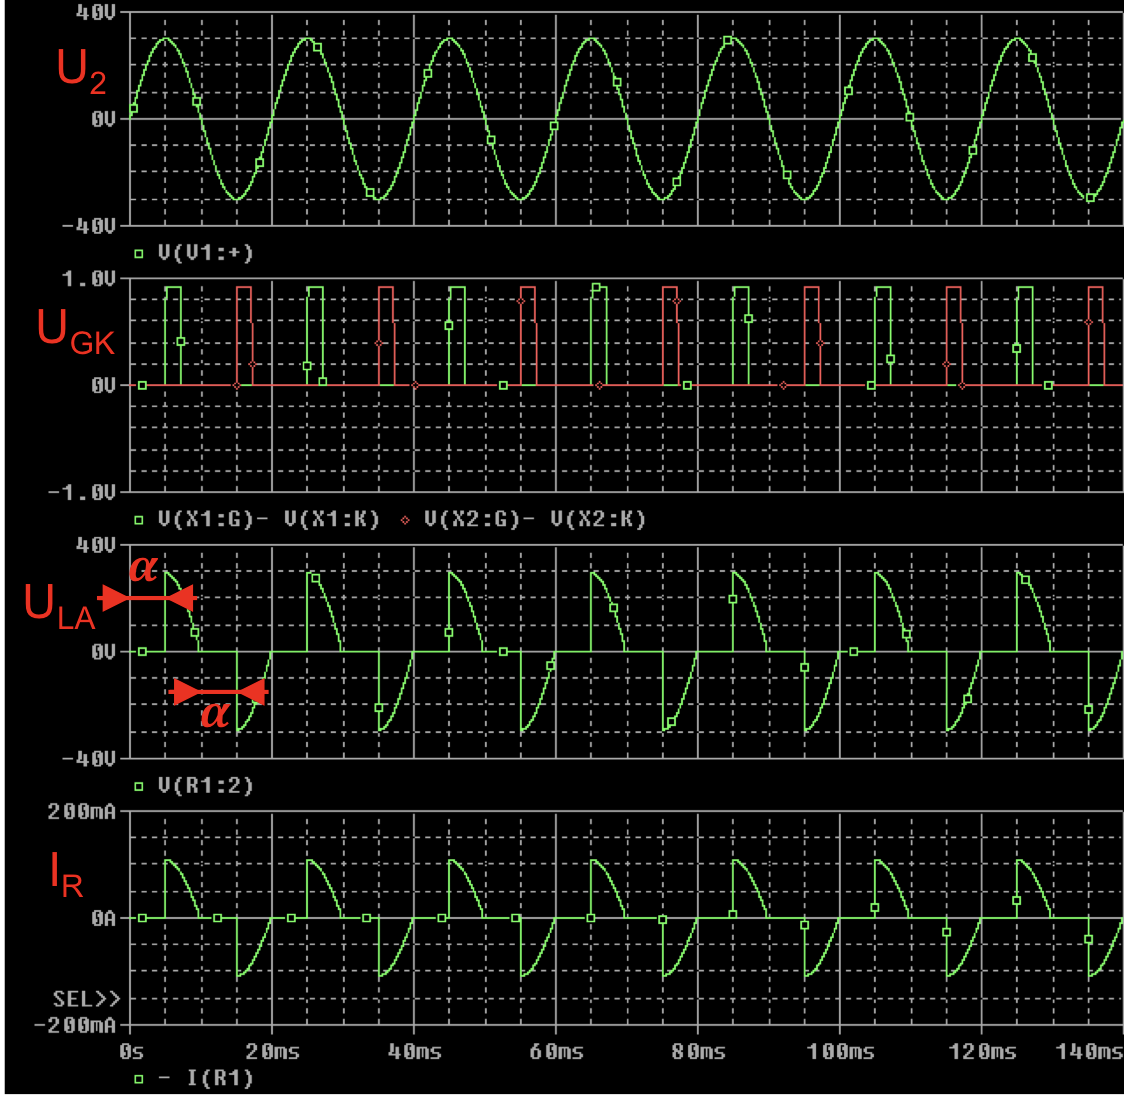
\includegraphics[width=0.85\linewidth]{images/Wechselstromsteller_Verlauf.png}
\end{center}
Eigenschaften:
\begin{itemize}
    \item Starke niederfrequente Harmonische.
    \item Abhängigkeit der Amplituden von $\alpha$.
    \item Ungerade und gerade Harmonische möglich.
\end{itemize}

\subsubsection{Rechteckwechselrichter}

Für symmetrische Rechteckspannung:
\[
\cbl{u(t) = \frac{4 U_{\mathrm{DC}}}{\pi}
\sum_{k=1,3,5,\dots}^{\infty} \frac{1}{k} \sin(k \omega t).}
\]

Eigenschaften:
\begin{itemize}
    \item Nur ungerade Harmonische.
    \item Amplituden $\sim 1/k$.
\end{itemize}

\subsubsection{PWM-Wechselrichter}

Eigenschaften:
\begin{itemize}
    \item Grundschwingung bei $f_1$.
    \item Seitenbänder um Vielfache der Schaltfrequenz $f_s$.
    \item Hochfrequente Harmonische dominieren.
\end{itemize}




\subsection{Effektivwert und Harmonische}

Der Gesamt-Effektivwert ergibt sich aus:
\[
\cbl{U_{\mathrm{RMS}}^2 = \sum_{n=1}^{\infty} U_{n,\mathrm{RMS}}^2.}
\]

Dabei:
\begin{itemize}
    \item $U_{1,\mathrm{RMS}}$: Grundschwingung
    \item $U_{n,\mathrm{RMS}}$: Harmonische Ordnung $n$
\end{itemize}

\subsection{Verzerrungsfaktor und THD}

\subsubsection{Total Harmonic Distortion (THD)}

Definition:
\[
\cbl{\mathrm{THD} =
\frac{\sqrt{ \sum_{n=2}^{\infty} U_{n,\mathrm{RMS}}^2 }}{U_{1,\mathrm{RMS}}}.}
\]

\paragraph{Leistungsfaktor bei nichtsinusförmigen Strömen}
\[
\lambda = \nu \cdot \cos\varphi_1 = \frac{U_{1,\mathrm{RMS}}}{U_{\mathrm{RMS}}} \cos\varphi_1
\]


Interpretation:
\begin{itemize}
    \item THD = 0: reiner Sinus
    \item THD gross: starke Verzerrung
\end{itemize}

\subsubsection{Verzerrungsfaktor}

\[
\cbl{\nu = \frac{U_{1,\mathrm{RMS}}}{U_{\mathrm{RMS}}}.}
\]

Beziehung:
\[
\cbl{\nu = \frac{1}{\sqrt{1 + \mathrm{THD}^2}}.}
\]

Dabei gilt:
\[
\nu = \frac{U_{1,\mathrm{RMS}}}{U_{\mathrm{RMS}}}
\]


\subsection{Wirkleistung und Harmonische}

Die Wirkleistung ergibt sich nur aus der Grundschwingung bei linearen Lasten:

\[
\cbl{P = U_{1,\mathrm{RMS}} \, I_{1,\mathrm{RMS}} \cos(\varphi_1).}
\]

Harmonische:
\begin{itemize}
    \item Erhöhen Effektivwert.
    \item Erzeugen Zusatzverluste.
    \item Tragen nicht zur Nutzleistung bei.
\end{itemize}

\crd{\textrightarrow\ Harmonische \textbf{verschlechtern Wirkungsgrad und Netzqualität}.}

\subsection{Filterwirkung der Last}

Bei R-L-Last:
\begin{itemize}
    \item Induktivität dämpft hohe Frequenzen.
    \item Strom ist sinusförmiger als Spannung.
\end{itemize}

Übertragungsfunktion:
\[
\cbl{|I_n| = \frac{|U_n|}{\sqrt{R^2 + (n \omega L)^2}}.}
\]

\paragraph{Stromharmonische bei R-L-Last}
Übertragungsfunktion der R--L-Last:
\[
\boxed{H(j\omega) = \frac{1}{R + j\omega L}}
\]
Stromamplitude der $n$-ten Harmonischen:
\[
I_n = \frac{U_n}{\sqrt{R^2 + (n\omega L)^2}}
\]


\subsection{Spektrale Bewertung von Umrichtern}

Typische Kenngrössen:
\begin{itemize}
    \item THD der Ausgangsspannung
    \item THD des Ausgangsstroms
    \item Oberwellenordnung mit maximaler Amplitude
    \item Anteil der Grundschwingung
\end{itemize}

\subsection{Typische Merksätze (Prüfungskern)}

\begin{itemize}
    \item \cbl{$U_{\mathrm{RMS}}^2 = \sum U_{n,\mathrm{RMS}}^2$}
    \item \cbl{$\mathrm{THD} = \dfrac{\sqrt{\sum_{n=2}^\infty U_n^2}}{U_1}$}
    \item Nur Grundschwingung liefert Wirkleistung.
    \item PWM verschiebt Harmonische in hohe Frequenzen.
\end{itemize}

\subsection{Typische Fehlerquellen}

\begin{itemize}
    \item Gesamt-$U_{\mathrm{RMS}}$ mit $U_{1,\mathrm{RMS}}$ verwechselt.
    \item THD mit Verzerrungsfaktor gleichgesetzt.
    \item Harmonische zur Wirkleistung addiert.
    \item Filterwirkung der Induktivität ignoriert.
\end{itemize}

\subsection{Minimal-Checkliste für Aufgaben}

\begin{enumerate}
    \item Signalform identifizieren (Rechteck, PWM, Anschnitt).
    \item Fourier-Koeffizienten bestimmen.
    \item Grundschwingung extrahieren.
    \item $U_{\mathrm{RMS}}$ aus Summenformel berechnen.
    \item THD berechnen.
    \item Einfluss der Lastinduktivität bewerten.
\end{enumerate}
